
Verschlüsselungsalgorithmen werden grundlegend in zwei Gruppen unterteilt.
Die erste Gruppe ist symmetrische Verschlüsselung, welche Grundlegend zum Verschlüsseln von Daten
oder Texten verwendet wird. Diese verwendet zum Ver\textendash\ und Entschlüssen den gleichen Schlüssel.
Im Gegensatz dazu steht die asymmetrische Verschlüsselung, welche zum Ver\textendash\ und Entschlüssen
zwei unterschiedliche Schlüssel verwendet. Diese werden Public Key (Verschlüsselung) und 
Private Key (Entschlüsselung) genannt. Als Beispiel, für einen Verwendungszweck von sowohl symmetrischer als auch 
asymmetrischer Verschlüsselung, ist folgend der HTTPS\textendash Verbindungsaufbau demonstriert.
\begin{figure}[h!]
    \centering
    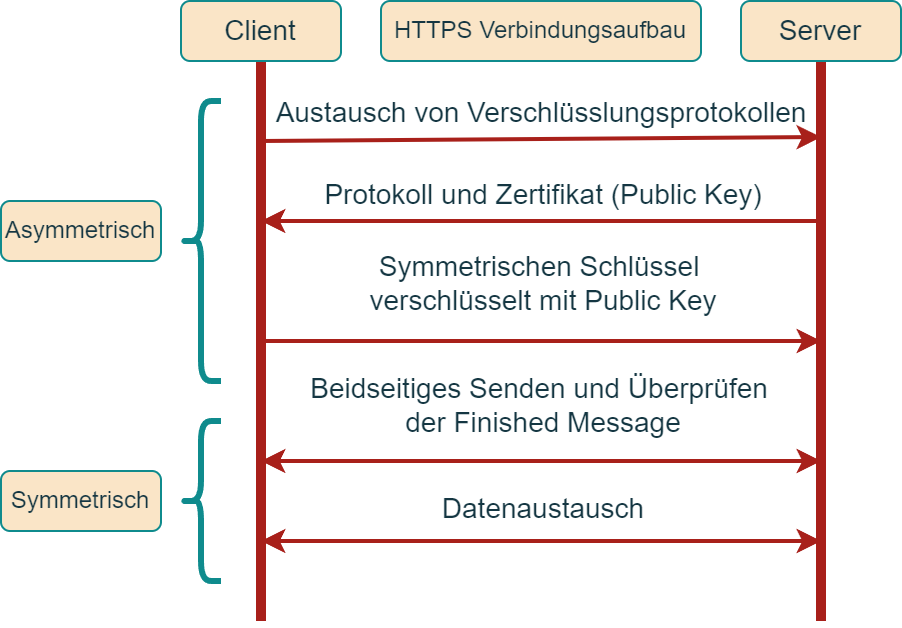
\includegraphics[width=0.45\textwidth]{sections/paul/https_verbindungsaufbau.drawio.png}
    \caption{Demonstration des HTTPS Verbindungsaufbaus}
    \label{fig:http_verbindungsaufbau}
\end{figure}
Wie in Abbildung~\ref{fig:http_verbindungsaufbau} dargestellt, erfolgt der Verbindungsaufbau, indem:
\begin{enumerate}
    \item Der Client unterstützte Verschlüsselungsalgorithmen an den Server sendet.
    \item Der Server das Sicherste der unterstützten Algorithmen auswählt und das Zertifikat, welches den Public Key enthält, an den Client sendet.
    \item Folgend generiert der Client einen symmetrischen Schlüssel, welcher mit dem Public Key des Servers verschlüsselt wird.
    \item Beide überprüfen die Integrität des Schlüssels gefolgt von der tatsächlichen Kommunikation.
\end{enumerate}

\subsection{Euklidischer Algorithmus: Beispiel zur Bestimmung des ggT}

Der Euklidische Algorithmus wird verwendet, um den größten gemeinsamen 
Teiler (ggT) zweier Zahlen effizient zu bestimmen. Anhand des Beispiels 
$N_1 = 132$ und $N_2 = 28$ wird der Algorithmus wie folgt angewendet:

\begin{enumerate}
    \item Schritt 1:
    Teile die größere Zahl durch die kleinere und bestimme den Rest:  
    \[
    132 \div 28 = 4 \, \text{Rest} \, 20 \quad \Rightarrow \quad 132 = 4 \cdot 28 + 20.
    \]

    \item Schritt 2:
    Die vorherige Divisorzahl $28$ wird der neue Dividend, und der Rest $20$ wird der neue Divisor:  
    \[
    28 \div 20 = 1 \, \text{Rest} \, 8 \quad \Rightarrow \quad 28 = 1 \cdot 20 + 8.
    \]

    \item Schritt 3:
    Wiederhole den Vorgang, bis der Rest $0$ wird:  
    \[
    20 \div 8 = 2 \, \text{Rest} \, 4 \quad \Rightarrow \quad 20 = 2 \cdot 8 + 4,
    \]  
    \[
    8 \div 4 = 2 \, \text{Rest} \, 0 \quad \Rightarrow \quad 8 = 2 \cdot 4 + 0.
    \]
\end{enumerate}

\subsection{RSA Algorithmus}
\subsubsection{Grundlegende Funktionsweise von RSA}
RSA ist ein verschlüsselt asymmetrisch und wird benötigt, um eine gesicherte Kommunikation 
zwischen mindestens zwei Parteien aufzubauen.
Andernfalls gäbe es keine Möglichkeit, den Schlüssel für die symmetrische Verschlüsselung \anf{abhörsicher} zu übertragen.
Die Sicherheit beruht darauf, dass die Faktorisierung von Primzahlen ein \anf{NP\textendash Hard} Problem ist\cite{moolchad_leveraging_nodate},
und damit nicht polynomieller Zeit gelöst werden kann. 

\subsubsection{Verschlüsselung mit RSA}
Die zwei Primfaktoren, welche für RSA benötigt werden, 
werden folgend mit $p$ und $q$ bezeichnet, wobei $p$ und $q$ relativ Prim zueinander sind. 
$n$ ist das Produkt dieser beiden Primfaktoren, welches bei derzeitigen RSA\textendash\ Implementierungen 
2048 Bit lang ist. Im folgenden Beispiel wird zur Nachvollziehbarkeit für $p$ und $q$ jeweils 13 und 17 gewählt, womit
$n = p \cdot q = 221$ ist. Als Zweites wird die Eulersche Phi\textendash\ Funktion benötigt, um 
\[
\phi(n) = (p-1) \cdot (q-1) = 12 \cdot 16 = 192
\]
zu berechnen. Folgend wird $e$ als Teil des Public Keys gewählt, wobei $e$ und $\phi(n)$ teilerfremd sind. In diesem 
Beispiel wird $e = 23$ gewählt. Der Public Key ist damit bereits vollständig: $(e, n) = (23, 221)$. Die letzte benötigte
Variable ist $d$, welche der erste Teil des Private Keys ist. $d$ ist das multiplikative Inverse zu $e$ modulo $\phi(n)$,
also die Zahl für die gilt:
\[
d \cdot e \equiv 1 \pmod{\phi(n)}
\]
In diesem Fall ist $d = 167$, da $167 \cdot 23 = 3841 \equiv 1 \pmod{192}$. Der Private Key ist damit $(d, n) = (167, 221)$.
Damit das Wort \anf{Dresden} tatsächlich verschlüsselt werden kann, wird dieses zu ASCII umgewandelt, wie in 
Tabelle \ref{tab:encryption_dresden} in den ersten beiden Spalten dargestellt.
Die Verschlüsselung erfolgt für jedes Zeichen einzeln durch:
\[
c = m^e \bmod n
\]
wobei $m$ der ASCII Code des zu verschlüsselnden Zeichens ist und $c$ der verschlüsselte Wert.
Für das Wort \anf{Dresden} ergibt sich die Verschlüsselung zu $[204, 160, 186, 123, 42, 186, 219]$, wie in Tabelle
\ref{tab:encryption_dresden} in den Spalten \anf{$m^e \bmod n$}  und \anf{$c$} dargestellt.
\begin{table}[h]
    \centering
    \begin{tabular}{|c|c|c|c|}
        \hline
        Buchstabe & m (ASCII) & $m^e \bmod n$ & $c$ \\
        \hline
        D & 68 & $68^{23} \bmod 221$ & 204 \\
        r & 114 & $114^{23} \bmod 221$ & 160 \\
        e & 101 & $101^{23} \bmod 221$ & 186 \\
        s & 115 & $115^{23} \bmod 221$ & 123 \\
        d & 100 & $100^{23} \bmod 221$ & 42 \\
        e & 101 & $101^{23} \bmod 221$ & 186 \\
        n & 110 & $110^{23} \bmod 221$ & 219 \\
        \hline
    \end{tabular}
    \caption{Verschlüsselung der einzelnen Buchstaben}
    \label{tab:encryption_dresden}
\end{table}

\subsubsection{Entschlüsselung mit RSA}
Die Entschlüsselung erfolgt analog mit dem Private Key ($d, n$) durch:
$ m = c^d \bmod n $
% wie in Tabelle \ref{tab:decryption_dresden} dargestellt ist.
% \begin{table}[H]
%    \centering
%    \begin{tabular}{|c|c|c|c|}
%        \hline
%        $c$ & $c^d \bmod n$ & m (ASCII) & Buchstabe \\
%        \hline
%        204 & $204^{167} \bmod 221$ & 68 & D \\
%        160 & $160^{167} \bmod 221$ & 114 & r \\
%        186 & $186^{167} \bmod 221$ & 101 & e \\
%        123 & $123^{167} \bmod 221$ & 115 & s \\
%        42 & $42^{167} \bmod 221$ & 100 & d \\
%        186 & $186^{167} \bmod 221$ & 101 & e \\
%        219 & $219^{167} \bmod 221$ & 110 & n \\
%        \hline
%    \end{tabular}
%    \caption{Entschlüsselung der einzelnen Buchstaben}
%    \label{tab:decryption_dresden}
% \end{table}
Die Nachricht \anf{Dresden} wurde damit erfolgreich ver\textendash\ und entschlüsselt.

\subsubsection{Welche Sicherheitsprobleme ergeben sich durch Quantencomputer?}
Sicherheitsprobleme, bezogen auf die 1. Forschungsfrage, ergeben sich durch die
Quantenkryptografie und speziell durch den Shors Algorithmus (Sektion \ref{sec:shor}).
Der Grund dafür liegt in der Annahme, dass Primfaktorzerlegung ein \anf{NP\textendash Hard} Problem ist und
damit nicht in deterministischer polynomieller Zeit gelöst werden kann. 
Genau das ist allerdings mit dem Shors Algorithmus möglich, da dieser die Periode anhand
einer Kongruenzgleichung bestimmt und dadurch mit dem größten gemeinsamen 
Teiler die Primfaktoren bestimmt.

% Python output
% p=13, q=17, n=221, phi=192, e=23, d=167
% Public Key: (23, 221)
% Private Key: (167, 221)
% Encrypting message: Dresden
% D[68] -> 68**23 % 221 = 204
% r[114] -> 114**23 % 221 = 160
% e[101] -> 101**23 % 221 = 186
% s[115] -> 115**23 % 221 = 123
% d[100] -> 100**23 % 221 = 42
% e[101] -> 101**23 % 221 = 186
% n[110] -> 110**23 % 221 = 219
% Decrypting message: [204, 160, 186, 123, 42, 186, 219]
% 204^167 % 221 = 68 -> D
% 160^167 % 221 = 114 -> r
% 186^167 % 221 = 101 -> e
% 123^167 % 221 = 115 -> s
% 42^167 % 221 = 100 -> d
% 186^167 % 221 = 101 -> e
% 219^167 % 221 = 110 -> n
% Original Message: Dresden
% Encrypted Message: [204, 160, 186, 123, 42, 186, 219]
% Decrypted Message: Dresden
